\documentclass[conference]{IEEEtran}
\IEEEoverridecommandlockouts
% The preceding line is only needed to identify funding in the first footnote. If that is unneeded, please comment it out.
\usepackage{cite}
\usepackage{amsmath,amssymb,amsfonts}
\usepackage{algorithmic}
\usepackage[dvipdfmx]{graphicx}
\usepackage[dvipdfmx]{color}
\usepackage{textcomp}
\usepackage{xcolor}

\def\BibTeX{{\rm B\kern-.05em{\sc i\kern-.025em b}\kern-.08em
    T\kern-.1667em\lower.7ex\hbox{E}\kern-.125emX}}
\begin{document}

\title{SuiteRec: Automatic Test Suite Recommendation System Using Code Clone Detection Tool\\
{\footnotesize \textsuperscript{*}Note: Sub-titles are not captured in Xplore and
should not be used}
\thanks{Identify applicable funding agency here. If none, delete this.}
}

\author{\IEEEauthorblockN{1\textsuperscript{st} Ryosuke Kurachi}
\IEEEauthorblockA{\textit{Information Science} \\
\textit{Nara Institute of Science and Technology}\\
Nara, Japan \\
kurachi.ryosuke.kp0@is.naist.jp}
\and
\IEEEauthorblockN{2\textsuperscript{nd} Eunjong Choi}
\IEEEauthorblockA{\textit{dept. name of organization (of Aff.)} \\
\textit{Kyoto Institute of Technology}\\
Kyoto, Japan \\
echoi@kit.ac.jp}
\and
\IEEEauthorblockN{3\textsuperscript{rd} Given Name Surname}
\IEEEauthorblockA{\textit{dept. name of organization (of Aff.)} \\
\textit{name of organization (of Aff.)}\\
City, Country \\
email address or ORCID}
\and
\IEEEauthorblockN{4\textsuperscript{th} Given Name Surname}
\IEEEauthorblockA{\textit{dept. name of organization (of Aff.)} \\
\textit{name of organization (of Aff.)}\\
City, Country \\
email address or ORCID}
\and
\IEEEauthorblockN{5\textsuperscript{th} Given Name Surname}
\IEEEauthorblockA{\textit{dept. name of organization (of Aff.)} \\
\textit{name of organization (of Aff.)}\\
City, Country \\
email address or ORCID}
\and
\IEEEauthorblockN{6\textsuperscript{th} Given Name Surname}
\IEEEauthorblockA{\textit{dept. name of organization (of Aff.)} \\
\textit{name of organization (of Aff.)}\\
City, Country \\
email address or ORCID}
}

\maketitle

\begin{abstract}
ソフトウェアの品質確保の要と言えるソフトウェアテストを支援することは重要です.これまでに,テスト作成コストを削減するために様々な自動生成技術が提案されてきました.しかし,自動生成されたテストコードはテスト対象コードの作成経緯や意図に基づいて生成されていないという性質から後のメンテナンス活動を困難にさせる課題があり,これは自動生成技術の実用的な利用の価値に疑問を提示させます.本研究では,この課題を解決するために,OSSに上に存在する既存の品質の高いテストコード推薦するツールSuiteRecを紹介します.SuiteRecは,類似コード検索ツールを用いてクローンペア間でのテスト再利用を考えます.入力コードに対して類似コードを検出し,その類似コードに対応するテストスイートを開発者に推薦します.さらに,テストコードの良くない実装を表すメトリクスであるテストスメルを開発者に提示し,より品質の高いテストスイートを推薦できるように推薦順位がランキングされています.提案ツールの評価では,被験者によってSuiteRecの使用した場合とそうでない場合でテストコードの作成してもらい,テスト作成をどの程度支援できるかを定量的および定性的に評価しました.その結果,(1) 条件分岐が多いプログラムのテストコードを作成する際にコードカバレッジの向上に効果的であること,(2) SuiteRecを使用して作成したテストコードは検出されたテストスメルの数が少なく品質が高いこと,(3) SuiteRecを使用してテストコードを作成した場合は使用しなかった場合と比べて開発者は,自身で作成したテストコードに自信が持てることが分かった.

%This document is a model and instructions for \LaTeX.
%This and the IEEEtran.cls file define the components of your paper [title, text, heads, etc.]. *CRITICAL: Do Not Use Symbols, Special Characters, Footnotes, 
%or Math in Paper Title or Abstract.
\end{abstract}

\begin{IEEEkeywords}
 clone detection, recommendation system, software testing, unit test 
\end{IEEEkeywords}

\section{Introduction}
近年,ソフトウェアに求められる要件が高度化・多様化する一方,ユーザからはソフトウェアの品質確保やコスト削減に対する要求も増加している[1].その中でも開発全体のコストに占める割合が大きく,品質確保の要ともいえるソフトウェアテストを支援する技術への関心が高まっている.しかし,現状では単体テスト作成作業の大部分が人手で行われており,多くのテストを作成しようとするとそれに比例してコストも増加してしまう.このような背景から,ソフトウェアの品質を確保しつつコスト削減を達成するために,様々な自動化技術が提案されている.

既存研究で提案されているEvoSuite[2]は,単体テスト自動生成における最先端のツールである.EvoSuiteは,対象コードを静的解析しプログラムを記号値で表現する.そして,対象コードの制御パスを通るような条件を集め,条件を満たす具体値を生成する.単体テストを自動生成することで,開発者は手作業での作成時間が自動生成によって節約することができ,またコードカバレッジを向上することができる.しかし,既存ツールによって自動生成されるテストコードは対象のコードの作成経緯や意図に基づいて生成されていないという性質から可読性が低く開発者に信用されていないことや後の保守作業を困難にするという課題がある[3].このことは、自動生成ツールの実用的な利用の価値に疑問を提示させる.テストが失敗するたびに,開発者はテスト対象のプログラム内での不具合を原因を特定するまたは,テスト自体を更新する必要があるかどうかを判断する必要がある.自動生成されたテストは,自動生成によって得られる時間の節約よりも読みづらく,保守作業に助けになるというよりかむしろ邪魔するという結果が報告されている.

本研究では,この課題を解決するためにOSSに存在する既存の品質の高いテストコード推薦するツールSuiteRecを紹介します.SuiteRecは類似コード検出ツールを用いてクローンペア間でのテスト再利用を考えます.入力コードに対して類似コードを検出し,その類似コードに対応するテストスイートを開発者に推薦します.さらに,テストコードの良くない実装を表すメトリクスであるテストスメルを開発者に提示し,より品質の高いテストスイートを推薦できるように推薦順位がランキングされています.

提案ツールの評価では,被験者によってSuiteRecの使用した場合とそうでない場合でテストコードの作成してもらい,テスト作成をどの程度支援できるかを定量的および定性的に評価した.その結果,提案ツールの利用は分岐が多く複雑なプログラムのテストスイートを作成する際に,コードカバレッジを向上させることができることや,ツールを使用して作成テストコードの品質が高いことが分かった.また,定性的な評価として実験後にアンケートを実施し,推薦ツールを使った場合多くの被験者は自分の作成したテストコードに自信が持てることが分かった.


\section{BACKGROUND AND RELETED WORK}
\textbf{Unit testing.}単体テストの実行タスクでは,ソフトウェアを動作させ,それぞれのテストケースにおいてソフトウェアが期待通りの振る舞いをするかを確認する.テスト工程のコスト削減のため,テスト実行タスクにおいて,単体テストではJUnitなどのテスト自動実行ツールの利用が産業界で進んでいる.しかし,テスト設計タスクは未だ手動で行うことが多く,自動化技術の実用化および普及が期待されている.

単体テスト設計タスクで作成されるテストケースは,テスト手順,テスト入力値,テスト期待結果から構成される.テスト手順に従ってテスト対象のソフトウェアにテスト入力値を与え,その出力結果をテスト期待結果と比較する.これが一致していればテストは合格となり,一致しなければ不合格となる.単体テスト設計タスクにおいては,多くの場合同値分割法,境界地分析法などのテストケース作成技法を用いてテスト入力値を作成するが,ソフトウェアの要求通りに動作するかを確認するために多くのバリエーションのテスト入力値を作成する必要がある.

\textbf{Test case generation.}既存の研究[4]は,既存のテストケースを再利用,自動生成,または再適用できることによって,ソフトウェア開発のテスト工程における時間とコストを大幅に節約できることを示している.テスト生成技術は,主にランダムテスト(RT),記号実行(SE),サーチベーステスト(SBST),モデルベース(MBT),組み合わせテストの5つに分類できる.SEはさらに静的記号実行(SSE)と動的記号実行(DSE)に分けられる.

RTとは,ソフトウェアにランダムな入力を与えるテスト手法である.無造作・均一にテストを実行するランダムテストは自動化に適しているが,コードカバレッジ率向上,バグ検出の観点において,テストケース1件当たりの効率は著しく悪い.

SEは対象コードを静的解析してプログラムを記号値で表現し,コード上のそれぞれのパスに対応する条件を抽出し,パスごとにパスを通るような入力値が満たすべき条件を集める.そして,パスごとにその条件をSMTソルバ[5]などの制約ソルバを用いて解き,得られた具体値をテスト入力値とする.

SBSTは,達成したい要件に対する達成度合いを定量的に評価できるように設計した評価関数に基づいて,ヒューリスティック探索アルゴリズムを用いて達成したい要件を満足するテストスイートを生成する技術の総称である.

MBTはモデルに基づいてテストスイートを生成する技術の総称である.モデルは何らかの形でテスト対象を記述したものであり,要求分析や設計のためのモデルを活用することもあれば,テストのためにモデルを作成することもある.

CTは,パラメータ間の相互作用に起因する不具合を効果的に発見するためにテストケースとしてパラメータに割り当てる値の組み合わせを生成する手法である.

\textbf{Test reuse using clone pairs.}

\textbf{Test Smell.}
プロダクションコードだけでなく,テストコードのも適切なプログラミングの慣習に従って設計する必要があります[44].テストコードのを適切に設計することの重要性は元々Beck[7]によって提唱されました.さらに,Van Deursenら[50]は11種類のテストスメルのカタログ,すなわちテストコードの良くない設計を表す実装とそれらを除去するためのリファクタリング技術を定義しました.このカタログはそれ以降,18個の新しいテスト臭を定義したMeszaros [42]によってより拡張されました。最近の研究では,テストスメルの存在は開発者のテストスイートの理解に悪い影響を与えるだけでなく,テストコードがプロダクションコード内の不具合を見つけるのにあまり効果的でなくなると言われています.

\section{SuiteRec}
SuiteRecは,開発者からの関数単位のコード片を入力とし,その入力コードの類似コードを検索します.そして類似コードに対応するテストスイートを優先順位の高い順に並び替え開発者に提示します.図は,テストスイートが推薦されるまでのステップを示しています.

\begin{figure}[htbp]
\centerline{\includegraphics[width=8.7cm]{SuiteRec2.pdf}}
\caption{Example of a figure caption.}
\label{fig}
\end{figure}

\begin{figure}[htbp]
\centerline{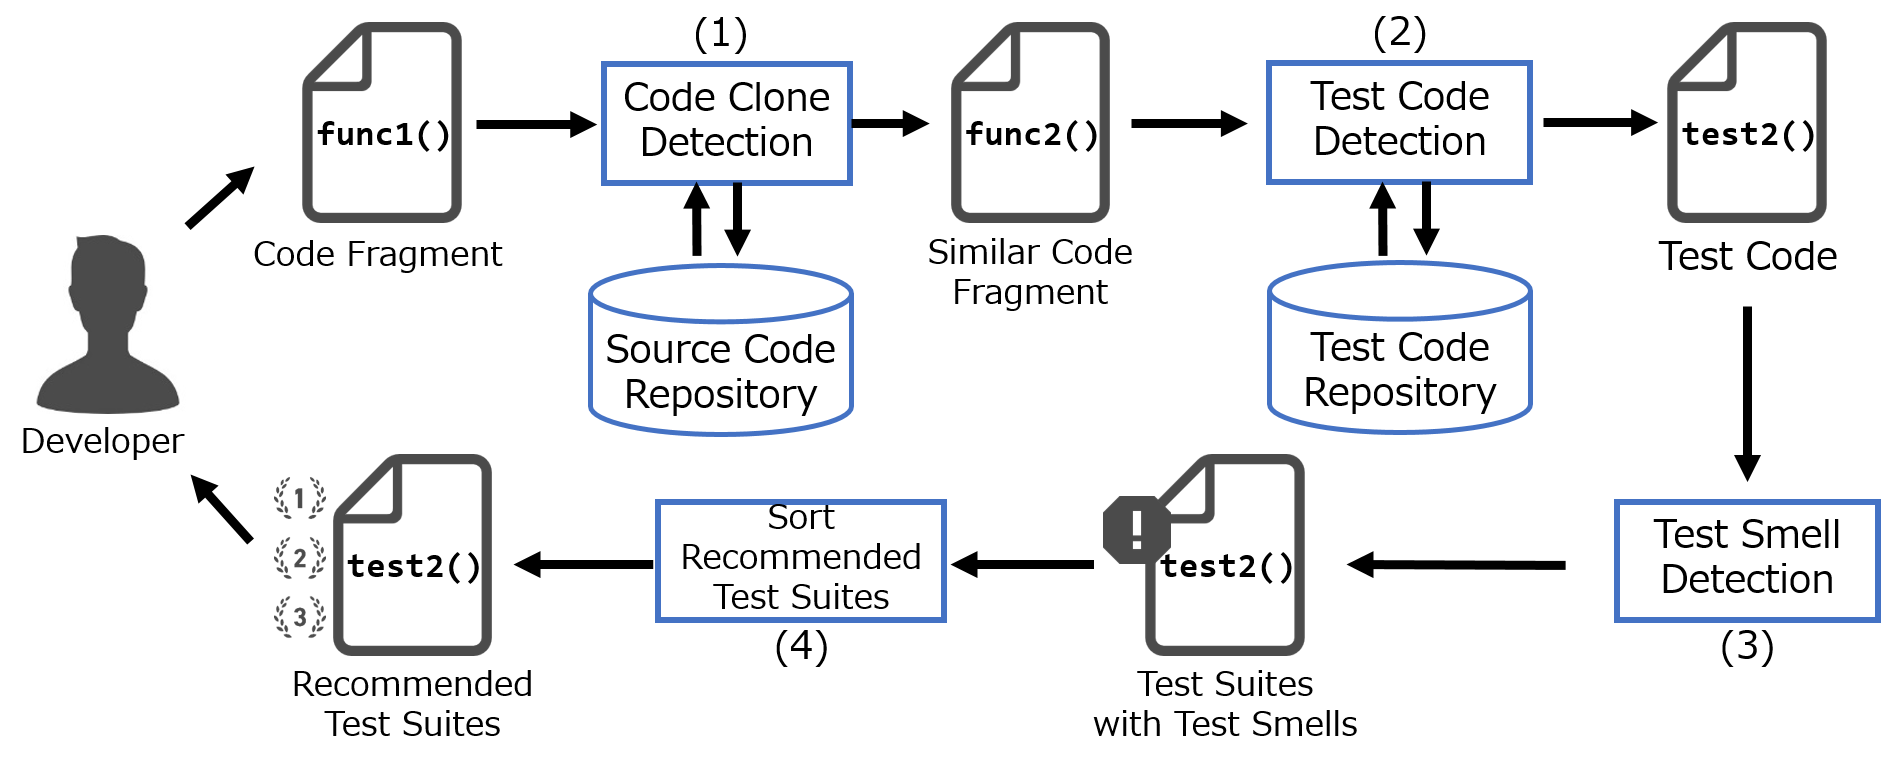
\includegraphics[width=8.5cm]{SuiteRec-OutLine.pdf}}
\caption{Example of a figure caption.}
\label{fig}
\end{figure}

\begin{enumerate}
\renewcommand{\labelenumi}{(\arabic{enumi})}
\item SuiteRecは,入力されたコード片を受け取ると,そのコード片をコードクローン検索ツールにかけ入力コード片の類似コードを検出します.
\item 複数の類似コード片が検出されると,次にその類似コード片に対応するテストスイートをテストコードリポジトリ内から検索します.
\item 各類似コード片のテストスイートが検出されると,次にそれらをテストスメル検出ツールにかけ各テストスイートに含まれるテストスメルを検出します
\item 最後に,1で得られた類似コードと入力コードの類似度と3で検出されたテストスメルの数を基に出力されるテストスイートの順番がランキングされる.
\end{enumerate}


\subsection{類似コード検索}
本研究では,類似コード検出ツールとしてNICADを採用した.NICADは検索対象のコードフラグメントのレイアウトを統一的に変換させ,行単位で関数単位のコードフラグメントを比較することで,クローンペア検出するツールであり,このような手法を取ることで,高精度・高再現率でのクローンペアの検出を実現している.NICADの標準の検出設定で提案ツールに実装した.

\subsection{テストコード検索}
類似コード片から対応するテストコードを検索するためにテスト対象コードとテストコードの対応付けを行う.本研究では,厳密にテストコードと対象コードを対応付けるために2つのステップを踏みます.

\begin{figure}[htbp]
\centerline{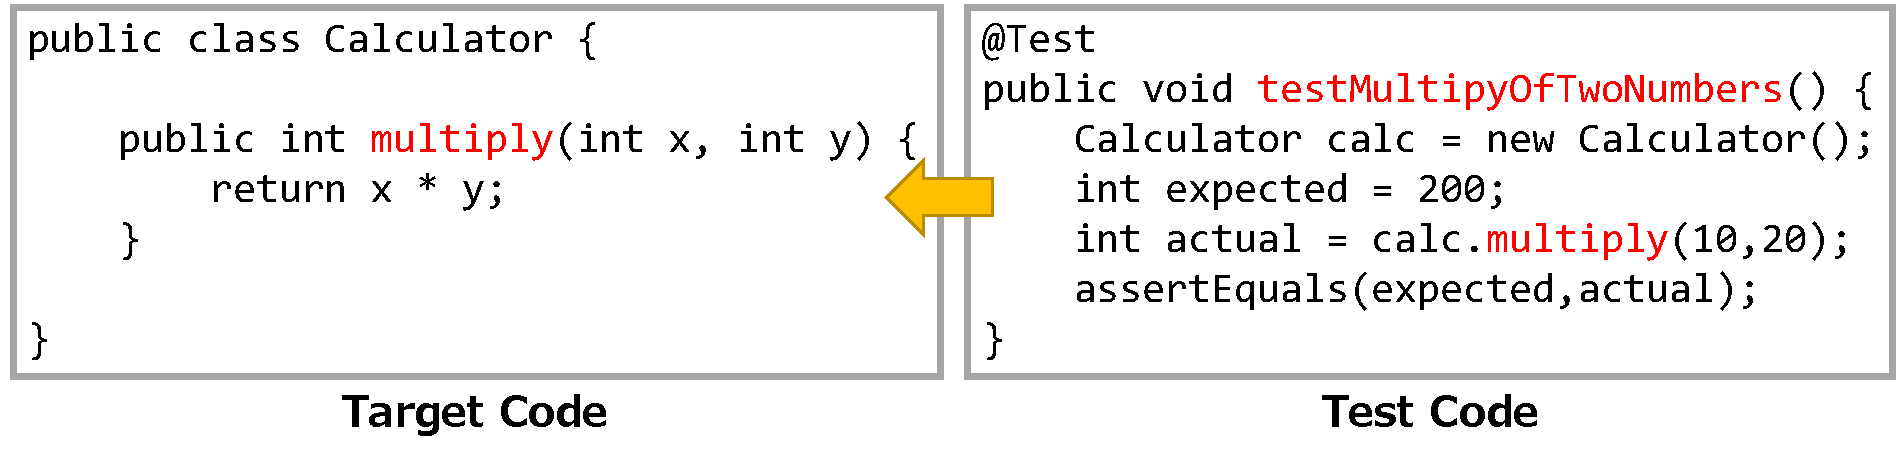
\includegraphics[width=8.5cm]{mapping.pdf}}
\caption{Example of a figure caption.}
\label{fig}
\end{figure}

\begin{enumerate}
\renewcommand{\labelenumi}{(\arabic{enumi})}
\item テストコードを静的解析し,メソッド呼び出しを確認
\item テストメソッドを区切り文字や大文字で分割し,対象メソッドと部分一致した時対応付ける
\end{enumerate}

単体テストでは,図の例のようにテストコード内でオブジェクトの生成が行い,テスト対象コードのメソッド呼び出して実行されます.すなわち,テストコードリポジトリ内のテストコードを静的解析し,メソッド呼び出しを取得することで,テスト対象コードとテストコードを対応付けます.ただ,テストメソッド内では複数のメソッドが呼び出されていることも考えられるのでさらに,メソッド名の比較も行います.テストメソッド名の記述方法としてテスト対象メソッドの処理の内容を忠実に表すことが推奨されており,対象メソッドの名前が記述されていることが多い.よってテストメソッドの名前を区切り文字や大文字で分割し,対象メソッドと部分一致した場合,対応付けるように実装した.

\subsection{テストスメルの検出}
本研究では,テストスメル検出ツールとしてtsDetect[6]を採用した.tsDetectはASTベースの検出手法で実装されたツールであり,19個のテストスメルを検出できるツールである.また,85%〜100%の精度と90%〜100%の再現率でテストスメルを正しく検出できることが報告されている.本研究では,tsDetectで検出できる19個のテストスメルの内テストコードの推薦を考える上で重要な以下の6種類のテストスメルを提示するように実装しました.

\begin{table}[hbtp]
\caption{Subject Test Smells}
\begin{tabular}{|c|p{5.5cm}|}
\hline
\textbf{Name}                   & \textbf{Description}                                                                                                       \\ \hline
\textbf{Assetion Roulette}        & 1つのテストメソッド内に複数のassert文が存在するテストコード.各assert文は異なる条件をテストするが,テストが失敗した場合開発者へ各assert文のエラーメッセージは提供されないので,失敗を特定することが困難になる.  \\ \hline
\textbf{Conditional Test Logic} &テストメソッド内に複数の制御文が含まれているテストスイート.テスト成功・失敗は制御フロー内にあるassert文に基づくの予測するのが難しい.                                                                                                                                                                                                           \\ \hline
\textbf{Default Test}            &JUnitなどのテスティングフレームワークを使用したテストコードの内,テストクラスやテストメソッドの名前がデフォルトの状態であるテストコード.テストコードの可読性の向上ために適切な名前に変更する必要がある.                                                                                                      \\ \hline
\textbf{Eager Test }             &テスト対象クラス内の複数のメソッドを呼び出しているテストコード.1つのテストメソッド内で複数のメソッド呼び出しを行うと,正確に何をテストしているかについて混乱が生じる.                                                                                                         \\ \hline
\textbf{Exception Handling}      & テストメソッド内で例外処理が含まれているまたは例外を投げるテストコード.例外処理はプロダクションコードに記述し,テストコード内で例外処理が正しく行われるかどうかを確かめるようにリファクタリングする必要がある.                                                                                                    \\ \hline
\textbf{Mystery Guest}          & テストメソッド内で、外部リソースを利用するテストコード.テストメソッド内だけで完結せず外部のファイルなど,外部リソースを利用すると外部との依存関係が生じ,外部リソースが壊れた場合テストも失敗してしまう.                                                                                                                \\ \hline
\end{tabular}
\end{table}


また,前処理として推薦テストコードとしてふさわしくない以下のテストスメルを含むテストコードを事前にテストコードリポジトリから削除し,推薦コードでとして出力されないようにした. 

\begin{itemize}
\item Empty Test
\item Ignored Test
\item Redundant Assertion
\item Unknow Test
\end{itemize}

\subsection{推薦ランキング}
入力コードと検出された類似コードの類似度とテストスイート内に含まれるテストスメルの数を基に推薦されるテストスイートの並び替えを行った.我々の以前の調査で,OSS上の有名プロジェクト内の両方のコードフラグメントにテストコードが存在するクローンペアを対象にプロダクションコードとなるクローンペアの類似度とそれに対応するテストコードの類似度を調査したところプロダクションコードの類似度が高いほど,テストコード間の類似度も高いことが分かっている.したがって,入力コードと類似コード間の類似度が高いクローンほどテストコードの再利用がしやすいと考える.SuiteRecではこの結果を基に類似度が高いクローンの順に並び替えさらに類似度が同じだった場合,テストスメルの数で順番を決めるような推薦ランキングを実装した.

\section{Evaluation}

このセクションでは,SuiteRecの定量的及び定性的に評価するために,被験者による実験結果を報告します.具体的には,以下のリサーチクエスチョンに答えて行きます.

\begin{itemize}
\item RQ1 : SuiteRecの利用は,開発者の作成したテストコードのカバレッジにどう影響するか?
\item RQ2 : SuiteRecの利用は,開発者のテストコード作成時間に影響するか?
\item RQ3 : SuiteRecの利用は,作成したテストコードの品質にどう影響するか?
\item RQ4 : SuiteRecの利用は,開発者のテストコード作成タスクの認識にどう影響しますか?
\end{itemize}

\subsection{Participant Selection}
我々は,基本的なプログラミングスキルを保有し,ソフトウェアテストに理解がある情報系の修士の学生10人対して行った.事前アンケートによると9割以上の学生が2年以上のプログラミング経験があり,8割以上の被験者が1年以上のJava言語の経験があった.また,すべての学生が授業などの講義でソフトウェアテストに関する基本的な知識を持っており,8割以上が単体テストの作成経験があった.

\subsection{Object Selection}
実験を行うために,3つのプロダクションコードを用意した.被験者はテストコードを作成するためプロダクションコードの仕様を十分理解していることが前提のため,我々はプロダクションコードとして競技プログラミングをよく用いられる典型的な数学の問題を選択した.また,その問題の仕様を確認できるように自然言語で書かれた仕様書を用意した.3つの各問題で違いを出すために問題1,2,3の順に条件分岐の数を8,16,24と多くなるように設定した.実験後のアンケートで,実験タスクについての理解を確認したがすべての被験者が実験タスクの理解についてポジティブな意見を述べたことが分かっている.また,十分な実験時間があったかどうかに関する質問に対してもネガティブな回答はなかった.したがって,被験者は与えられた実験タスクに対して十分に理解し,作業時間も十分にあったことが分かる.

\begin{figure}[htbp]
\centerline{\includegraphics[width=8.5cm]{src.pdf}}
\caption{Example of a figure caption.}
\label{fig}
\end{figure}

\subsection{Experiment Procedure}
まず初めにソフトウェアテストに関する基本的な知識からJUnitを使用に関する30分の講義と練習問題を実施し,テストコードの記述に対する理解を確認した.そして本番の実験課題の3つのプロダクションコードのテストコードを作成してもらった.実験タスクの終了は被験者に判断してもらう.具体的には,被験者自身が作成したテストコードのカバレッジ・品質に満足した時,実験タスクを終了してもらった.実験時間は1問につき最大25分の時間を設けた.推薦ツールの利用効果が問題によって偏らないように,被験者によってツールを利用の有無を問題によって変えるように割り当てた.また,推薦ツールを利用した場合の学習効果を防ぐために,3つの問題で連続してツールを利用しないようにタスクの割り当てを行った.また,過去の回答を参考にできないようにした.

\section{Results}

このセクションでは,10人の被験者によるSuiteRecの定量的および定性的評価結果を報告する.前のセクションで説明したように,4つの研究課題について分析結果を提示します.

\subsection{RQ1: SuiteRecの利用は,開発者の作成したテストコードのカバレッジにどう影響するか?}
本実験では,被験者によって提出されたテストスイートの命令網羅と分岐網羅の2種類のコードカバレッジの計算した.カバレッジの計算には統合開発環境Eclipseのプラグインとして搭載されているEclEmmaを利用した.図1と図2はそれぞれ被験者による命令網羅と分岐網羅の割合を示す.結果として,命令網羅の割合は3つの問題すべてにおいてツールを利用した場合とそうでない場合で網羅率にほとんど違いはなく,どの問題も網羅率が90\%を超えている.図2の分岐網羅についても分岐数が少ないTASK1とTASK2についてはツールを使用した場合とそうでない場合でほとんど差がないことが分かる.しかし,プロダクションコードの分岐数が最も多いTASK3については,実験者の平均カバレッジに10\%以上の差があることが分かった.この結果は,分岐が多いプロダクションコードのテストコードを作成する際に,SuiteRecで推薦されるテストコードは網羅率を向上するのに役に立つことが考えられる.実際に実験後のアンケートの記述欄には,推薦コードによって見落としていたテスト項目をフォローすることができたという報告が複数存在した.
\begin{figure}[htbp]
\centerline{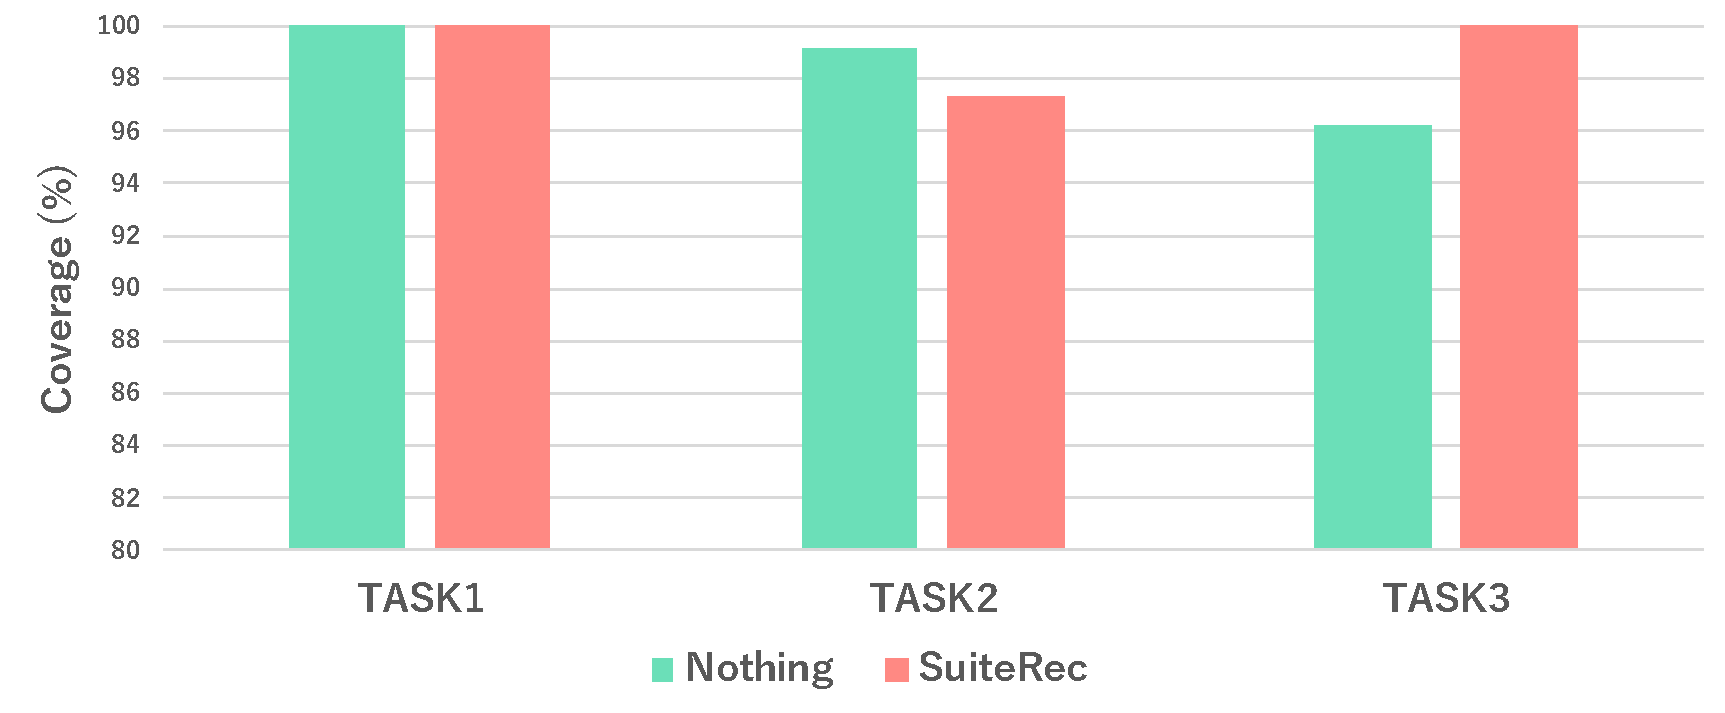
\includegraphics[width=8.5cm]{C0.pdf}}
\caption{Example of a figure caption.}
\label{fig}
\end{figure}

\begin{figure}[htbp]
\centerline{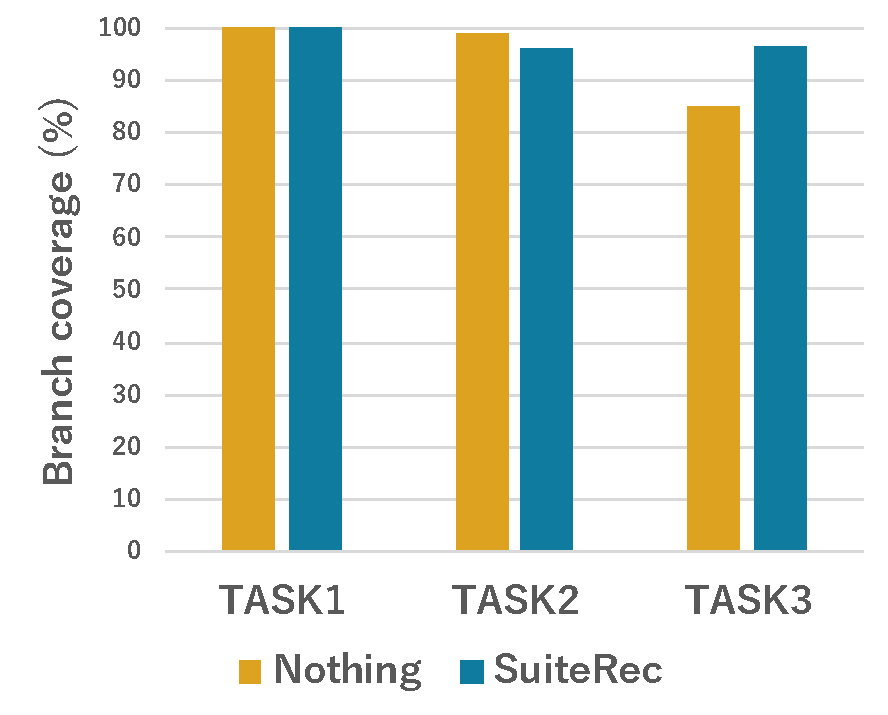
\includegraphics[width=8.5cm]{C1.pdf}}
\caption{Example of a figure caption.}
\label{fig}
\end{figure}

\subsection{RQ2: SuiteRecの利用は,開発者のテストコード作成時間に影響するか?}

図5は,SuiteRecを使用した場合と何も使用しない場合で,テストコード作成タスクの終了までに費やされた時間を比較しています.3つの問題の内,2つの問題でSuiteRecを使用した場合そうでない場合と比べてテスト作成時間が大きくなっていることが分かる.この結果はSuiteRecによって推薦される複数のテストスイートを読み理解するのに時間がかかる可能性があります.被験者は,推薦されるテストコードをそのままの形で再利用することができません.入力したプロダクションコードと検出された類似コードの差分を見てテストコードを書き換える必要があります.また,実験後のアンケートではテスト対象のオブジェクト生成の記述を再利用する際にその都度書き換える必要があり,時間がかかってしまったと述べている.問題2については,SuiteRecを利用した場合の方がテスト作成時間が短いことが分かる.我々は,提出されたテストコード調査したところカバレッジに差はないもののSuiteRecを使用しない場合はテストケース(項目)の数多くなっていることが分かった.この結果は,被験者は無駄なテストケースを多く記述するのに無駄な時間を費やしてしまった可能性がある.
\begin{figure}[htbp]
\centerline{\includegraphics[width=8.5cm]{time.pdf}}
\caption{Example of a figure caption.}
\label{fig}
\end{figure}

\subsection{RQ3 : SuiteRecの利用は,作成したテストコードの品質にどう影響するか?}

図6はSuiteRecを使用した場合とそうでない場合で,提出されたテストコード内のテストスメル数を比較しています.すべてのTASKに対して,SuiteRecを使用して作成されたテストコードはテストスメルをあまり含んでいないことが分かる.この結果は,推薦されるテストコード自体の品質が高く開発者はそれを再利用することで品質を維持したままテストコードを作成したと考えられる.また,ツールの出力画面で推薦されるテストスイート内に含まれているテストスメルを提示することで,それを基にテストコードを書き替えより品質が高いテストコードを提出した可能性が考えられる.実際のアンケートの記述でも提示されたテストスメルを理解し,それをなくすようにリファクタリングしテストコードを作成したという報告がされている.一方で,テストスメルが含まれていることは気づいていたがリファクタリングの方法が分からずそのまま提出したと述べている被験者も存在した.これは今後のツールの課題であり,テストスメルのリファクタリング方法も提示する改良の必要がある.SuiteRecを使用しなかった場合は,使用した場合と比べ全体として5倍以上の被験者はテストスメルを埋め込んでいた.その中でも多く埋め込まれていたテストスメルとして,Assertion Roulette, Default Test, Eager Testが挙げられる.多くの被験者は,初期状態のテストメソッドの名前を変更せず一つのテストメソッド内でコピーアンドペーストによってAssert文を記述していたのが原因だと考えられる.実際に既存研究でもこれらのテストスメルが既存プロジェクトで多く検出されていることが報告されている. 

\begin{figure}[htbp]
\centerline{\includegraphics[width=8.5cm]{testsmell.pdf}}
\caption{Example of a figure caption.}
\label{fig}
\end{figure}

\subsection{RQ4 : SuiteRecの利用は,開発者のテストコード作成タスクの認識にどう影響しますか?}


\begin{figure*}[t]
 \begin{center}
  \includegraphics[width=18.5cm]{SuiteRec_qa_result.pdf}
  \caption{キャプション}
  \label{}
 \end{center}
\end{figure*}



%\subsection{Maintaining the Integrity of the Specifications}

The IEEEtran class file is used to format your paper and style the text. All margins, 
column widths, line spaces, and text fonts are prescribed; please do not 
alter them. You may note peculiarities. For example, the head margin
measures proportionately more than is customary. This measurement 
and others are deliberate, using specifications that anticipate your paper 
as one part of the entire proceedings, and not as an independent document. 
Please do not revise any of the current designations.

\section{Prepare Your Paper Before Styling}
Before you begin to format your paper, first write and save the content as a 
separate text file. Complete all content and organizational editing before 
formatting. Please note sections \ref{AA}--\ref{SCM} below for more information on 
proofreading, spelling and grammar.

Keep your text and graphic files separate until after the text has been 
formatted and styled. Do not number text heads---{\LaTeX} will do that 
for you.

\subsection{Abbreviations and Acronyms}\label{AA}
Define abbreviations and acronyms the first time they are used in the text, 
even after they have been defined in the abstract. Abbreviations such as 
IEEE, SI, MKS, CGS, ac, dc, and rms do not have to be defined. Do not use 
abbreviations in the title or heads unless they are unavoidable.

\subsection{Units}
\begin{itemize}
\item Use either SI (MKS) or CGS as primary units. (SI units are encouraged.) English units may be used as secondary units (in parentheses). An exception would be the use of English units as identifiers in trade, such as ``3.5-inch disk drive''.
\item Avoid combining SI and CGS units, such as current in amperes and magnetic field in oersteds. This often leads to confusion because equations do not balance dimensionally. If you must use mixed units, clearly state the units for each quantity that you use in an equation.
\item Do not mix complete spellings and abbreviations of units: ``Wb/m\textsuperscript{2}'' or ``webers per square meter'', not ``webers/m\textsuperscript{2}''. Spell out units when they appear in text: ``. . . a few henries'', not ``. . . a few H''.
\item Use a zero before decimal points: ``0.25'', not ``.25''. Use ``cm\textsuperscript{3}'', not ``cc''.)
\end{itemize}

\subsection{Equations}
Number equations consecutively. To make your 
equations more compact, you may use the solidus (~/~), the exp function, or 
appropriate exponents. Italicize Roman symbols for quantities and variables, 
but not Greek symbols. Use a long dash rather than a hyphen for a minus 
sign. Punctuate equations with commas or periods when they are part of a 
sentence, as in:
\begin{equation}
a+b=\gamma\label{eq}
\end{equation}

Be sure that the 
symbols in your equation have been defined before or immediately following 
the equation. Use ``\eqref{eq}'', not ``Eq.~\eqref{eq}'' or ``equation \eqref{eq}'', except at 
the beginning of a sentence: ``Equation \eqref{eq} is . . .''

\subsection{\LaTeX-Specific Advice}

Please use ``soft'' (e.g., \verb|\eqref{Eq}|) cross references instead
of ``hard'' references (e.g., \verb|(1)|). That will make it possible
to combine sections, add equations, or change the order of figures or
citations without having to go through the file line by line.

Please don't use the \verb|{eqnarray}| equation environment. Use
\verb|{align}| or \verb|{IEEEeqnarray}| instead. The \verb|{eqnarray}|
environment leaves unsightly spaces around relation symbols.

Please note that the \verb|{subequations}| environment in {\LaTeX}
will increment the main equation counter even when there are no
equation numbers displayed. If you forget that, you might write an
article in which the equation numbers skip from (17) to (20), causing
the copy editors to wonder if you've discovered a new method of
counting.

{\BibTeX} does not work by magic. It doesn't get the bibliographic
data from thin air but from .bib files. If you use {\BibTeX} to produce a
bibliography you must send the .bib files. 

{\LaTeX} can't read your mind. If you assign the same label to a
subsubsection and a table, you might find that Table I has been cross
referenced as Table IV-B3. 

{\LaTeX} does not have precognitive abilities. If you put a
\verb|\label| command before the command that updates the counter it's
supposed to be using, the label will pick up the last counter to be
cross referenced instead. In particular, a \verb|\label| command
should not go before the caption of a figure or a table.

Do not use \verb|\nonumber| inside the \verb|{array}| environment. It
will not stop equation numbers inside \verb|{array}| (there won't be
any anyway) and it might stop a wanted equation number in the
surrounding equation.

\subsection{Some Common Mistakes}\label{SCM}
\begin{itemize}
\item The word ``data'' is plural, not singular.
\item The subscript for the permeability of vacuum $\mu_{0}$, and other common scientific constants, is zero with subscript formatting, not a lowercase letter ``o''.
\item In American English, commas, semicolons, periods, question and exclamation marks are located within quotation marks only when a complete thought or name is cited, such as a title or full quotation. When quotation marks are used, instead of a bold or italic typeface, to highlight a word or phrase, punctuation should appear outside of the quotation marks. A parenthetical phrase or statement at the end of a sentence is punctuated outside of the closing parenthesis (like this). (A parenthetical sentence is punctuated within the parentheses.)
\item A graph within a graph is an ``inset'', not an ``insert''. The word alternatively is preferred to the word ``alternately'' (unless you really mean something that alternates).
\item Do not use the word ``essentially'' to mean ``approximately'' or ``effectively''.
\item In your paper title, if the words ``that uses'' can accurately replace the word ``using'', capitalize the ``u''; if not, keep using lower-cased.
\item Be aware of the different meanings of the homophones ``affect'' and ``effect'', ``complement'' and ``compliment'', ``discreet'' and ``discrete'', ``principal'' and ``principle''.
\item Do not confuse ``imply'' and ``infer''.
\item The prefix ``non'' is not a word; it should be joined to the word it modifies, usually without a hyphen.
\item There is no period after the ``et'' in the Latin abbreviation ``et al.''.
\item The abbreviation ``i.e.'' means ``that is'', and the abbreviation ``e.g.'' means ``for example''.
\end{itemize}
An excellent style manual for science writers is \cite{b7}.

\subsection{Authors and Affiliations}
\textbf{The class file is designed for, but not limited to, six authors.} A 
minimum of one author is required for all conference articles. Author names 
should be listed starting from left to right and then moving down to the 
next line. This is the author sequence that will be used in future citations 
and by indexing services. Names should not be listed in columns nor group by 
affiliation. Please keep your affiliations as succinct as possible (for 
example, do not differentiate among departments of the same organization).

\subsection{Identify the Headings}
Headings, or heads, are organizational devices that guide the reader through 
your paper. There are two types: component heads and text heads.

Component heads identify the different components of your paper and are not 
topically subordinate to each other. Examples include Acknowledgments and 
References and, for these, the correct style to use is ``Heading 5''. Use 
``figure caption'' for your Figure captions, and ``table head'' for your 
table title. Run-in heads, such as ``Abstract'', will require you to apply a 
style (in this case, italic) in addition to the style provided by the drop 
down menu to differentiate the head from the text.

Text heads organize the topics on a relational, hierarchical basis. For 
example, the paper title is the primary text head because all subsequent 
material relates and elaborates on this one topic. If there are two or more 
sub-topics, the next level head (uppercase Roman numerals) should be used 
and, conversely, if there are not at least two sub-topics, then no subheads 
should be introduced.

\subsection{Figures and Tables}
\paragraph{Positioning Figures and Tables} Place figures and tables at the top and 
bottom of columns. Avoid placing them in the middle of columns. Large 
figures and tables may span across both columns. Figure captions should be 
below the figures; table heads should appear above the tables. Insert 
figures and tables after they are cited in the text. Use the abbreviation 
``Fig.~\ref{fig}'', even at the beginning of a sentence.

\begin{table}[htbp]
\caption{Table Type Styles}
\begin{center}
\begin{tabular}{|c|c|c|c|}
\hline
\textbf{Table}&\multicolumn{3}{|c|}{\textbf{Table Column Head}} \\
\cline{2-4} 
\textbf{Head} & \textbf{\textit{Table column subhead}}& \textbf{\textit{Subhead}}& \textbf{\textit{Subhead}} \\
\hline
copy& More table copy$^{\mathrm{a}}$& &  \\
\hline
\multicolumn{4}{l}{$^{\mathrm{a}}$Sample of a Table footnote.}
\end{tabular}
\label{tab1}
\end{center}
\end{table}

\begin{figure}[htbp]
\centerline{\includegraphics{fig1.pdf}}
\caption{Example of a figure caption.}
\label{fig}
\end{figure}

Figure Labels: Use 8 point Times New Roman for Figure labels. Use words 
rather than symbols or abbreviations when writing Figure axis labels to 
avoid confusing the reader. As an example, write the quantity 
``Magnetization'', or ``Magnetization, M'', not just ``M''. If including 
units in the label, present them within parentheses. Do not label axes only 
with units. In the example, write ``Magnetization (A/m)'' or ``Magnetization 
\{A[m(1)]\}'', not just ``A/m''. Do not label axes with a ratio of 
quantities and units. For example, write ``Temperature (K)'', not 
``Temperature/K''.

\section*{Acknowledgment}

The preferred spelling of the word ``acknowledgment'' in America is without 
an ``e'' after the ``g''. Avoid the stilted expression ``one of us (R. B. 
G.) thanks $\ldots$''. Instead, try ``R. B. G. thanks$\ldots$''. Put sponsor 
acknowledgments in the unnumbered footnote on the first page.

\section*{References}

Please number citations consecutively within brackets \cite{b1}. The 
sentence punctuation follows the bracket \cite{b2}. Refer simply to the reference 
number, as in \cite{b3}---do not use ``Ref. \cite{b3}'' or ``reference \cite{b3}'' except at 
the beginning of a sentence: ``Reference \cite{b3} was the first $\ldots$''

Number footnotes separately in superscripts. Place the actual footnote at 
the bottom of the column in which it was cited. Do not put footnotes in the 
abstract or reference list. Use letters for table footnotes.

Unless there are six authors or more give all authors' names; do not use 
``et al.''. Papers that have not been published, even if they have been 
submitted for publication, should be cited as ``unpublished'' \cite{b4}. Papers 
that have been accepted for publication should be cited as ``in press'' \cite{b5}. 
Capitalize only the first word in a paper title, except for proper nouns and 
element symbols.

For papers published in translation journals, please give the English 
citation first, followed by the original foreign-language citation \cite{b6}.

\begin{thebibliography}{00}
\bibitem{b1} G. Eason, B. Noble, and I. N. Sneddon, ``On certain integrals of Lipschitz-Hankel type involving products of Bessel functions,'' Phil. Trans. Roy. Soc. London, vol. A247, pp. 529--551, April 1955.
\bibitem{b2} J. Clerk Maxwell, A Treatise on Electricity and Magnetism, 3rd ed., vol. 2. Oxford: Clarendon, 1892, pp.68--73.
\bibitem{b3} I. S. Jacobs and C. P. Bean, ``Fine particles, thin films and exchange anisotropy,'' in Magnetism, vol. III, G. T. Rado and H. Suhl, Eds. New York: Academic, 1963, pp. 271--350.
\bibitem{b4} K. Elissa, ``Title of paper if known,'' unpublished.
\bibitem{b5} R. Nicole, ``Title of paper with only first word capitalized,'' J. Name Stand. Abbrev., in press.
\bibitem{b6} Y. Yorozu, M. Hirano, K. Oka, and Y. Tagawa, ``Electron spectroscopy studies on magneto-optical media and plastic substrate interface,'' IEEE Transl. J. Magn. Japan, vol. 2, pp. 740--741, August 1987 [Digests 9th Annual Conf. Magnetics Japan, p. 301, 1982].
\bibitem{b7} M. Young, The Technical Writer's Handbook. Mill Valley, CA: University Science, 1989.
\end{thebibliography}
\vspace{12pt}
\color{red}
IEEE conference templates contain guidance text for composing and formatting conference papers. Please ensure that all template text is removed from your conference paper prior to submission to the conference. Failure to remove the template text from your paper may result in your paper not being published.

\end{document}
